\subsection{Mecánica de juego.}
El siguiente apartado que aportó información significativa al diseño del juego, 
fue el de la Mecánica del juego, pues en éste se definieron aspectos técnicos 
que garantizarían el funcionamiento de la mecánica de juego descrita en el 
primer apartado, tales como la cámara, los periféricos, los controles y el 
guardado y carga de datos. 
\\
\par
La cámara se definió como una cámara de perspectiva ortogonal lateral que seguiría 
el movimiento en ambos ejes coordenados (Ver figura \ref{fig:Camara}).

\begin{figure}
  \centering
  \subfigure[Seguimiento horizontal]{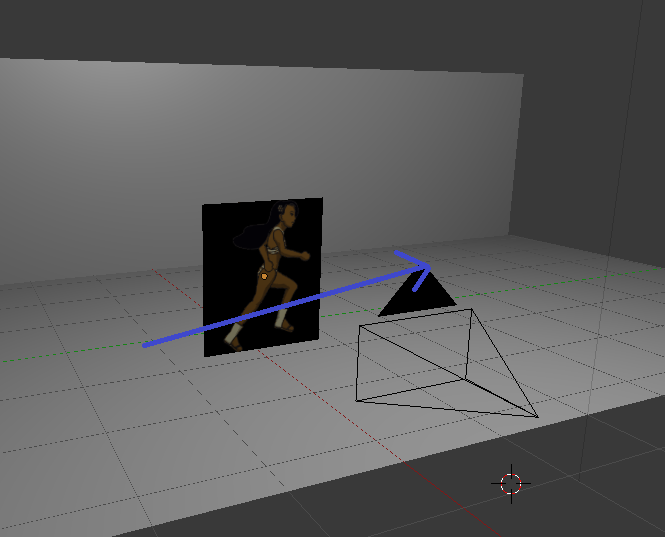
\includegraphics[width=0.7 \textwidth]{05TrabajoRealizado/01DocDiseno02/imagenes/camara01}}
   \subfigure[Seguimiento vertical.]{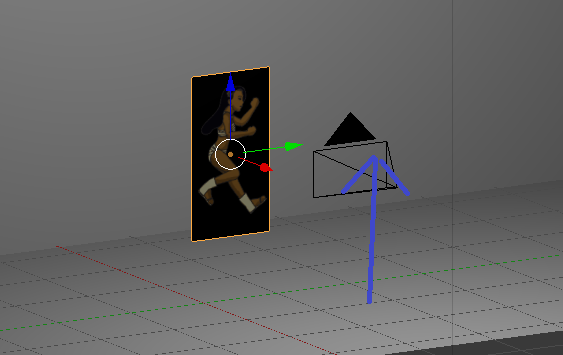
\includegraphics[width=0.7 \textwidth]{05TrabajoRealizado/01DocDiseno02/imagenes/camara02}}
  \caption{La cámara seguirá la posición del jugador en el eje x y y.}
  \label{fig:Camara}
\end{figure} 
 

\par
Por su parte, los controles del juego se establecieron como un conjunto de cuatro 
botones (Ver figura \ref{fig:GUI} ); cada uno con una acción específica a 
desempeñar: mover hacia la izquierda, mover hacia la derecha, disparar, hablar, 
saltar. Siendo periférico o el medio de interacción de los botones y el jugador 
la pantalla táctil del teléfono.  

\begin{figure}
				\centering
				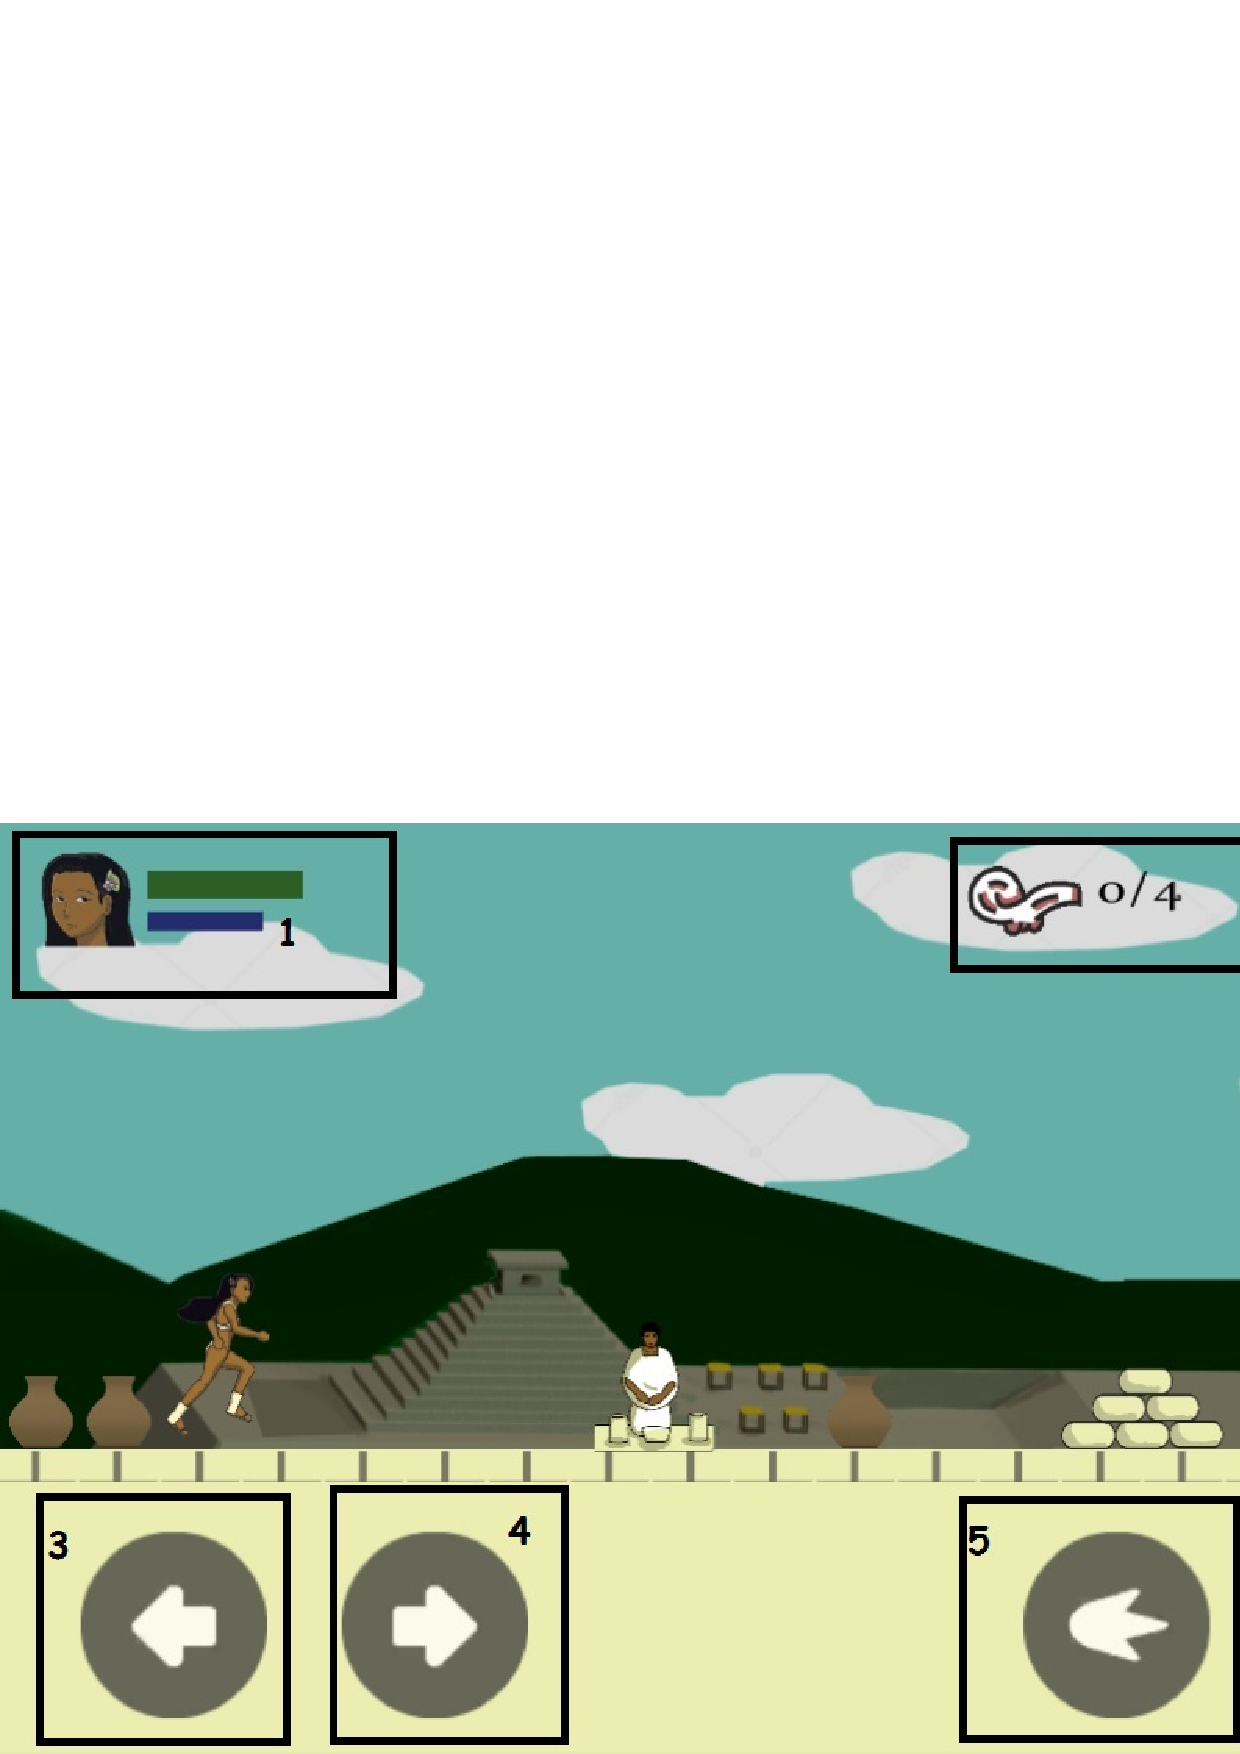
\includegraphics[height=0.3 \textheight]{05TrabajoRealizado/01DocDiseno02/imagenes/ControlCorrerDer}
				\caption{1 Información del personaje jugable, barra verde indicador 
				de la cantidad de vida, barra azul cantidad de tonalli. 2 Objetivos 
				del nivel o información útil. 3 Botón moverse izquierda. 4 Botón 
				moverse derecha. 5 Botón disparar tonalli. 6 Botón saltar.}
				\label{fig:GUI}
\end{figure}


\par
En cuanto al guardado y la carga, se propusieron dos tipos guardado y carga automática 
y guardado y carga de checkpoint; el primero guarda el progreso del jugador al 
completar el nivel y permite inicializar los niveles desbloqueados y el segundo 
se utiliza dentro de un nivel para guardar el progreso del jugador en el nivel 
en caso de que muera pueda iniciar desde el último checkpoint que tocó. 
Si el lector de este documento dese profundizar más en lo anteriormente dicho, 
se le recomienda consultar el Capítulo 5 del documento de diseño.